% Projeckt z předmětu INC
% Autor: Martin Slezák

\documentclass{article}

\usepackage[czech]{babel}

\usepackage[letterpaper,top=2cm,bottom=2cm,left=3cm,right=3cm,marginparwidth=1.75cm]{geometry}

% Useful packages
\usepackage{amsmath}
\usepackage{graphicx}
\usepackage[colorlinks=true, allcolors=blue]{hyperref}

\title{Výstupní zpráva}
\author{Martin Slezák \\ xsleza26}
\date{\today}

\begin{document}
\maketitle

	\section{Architektura navrženého obvodu}
	\subsection{Schéma obvodu}
	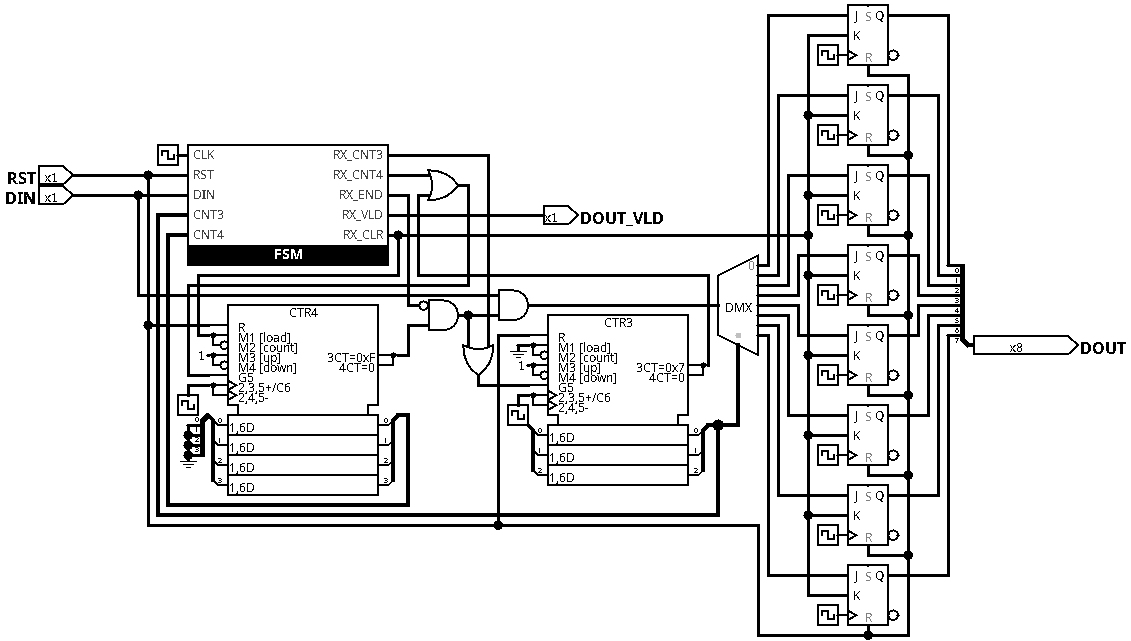
\includegraphics[scale=0.5778]{"./src/rlc.png"}

	\subsection{Popis obvodu}

\end{document}

%%%%% Projekt z předmětu IEL %%%% 
%% Autor: Martin Slezák

%\documentclass[]{fitiel}
%\usepackage{svg}

% implicitní cesta k obrázkům
%\graphicspath{{fig/}}

% hlavička 
% příkaz logo - vkládá logo fakulty dle zvoleného jazyka
%\title{\logo\\IEL -- protokol k projektu}
%\author{Martin, Slezák \\ xsleza26}
%\date{\today} % today - dnešní datum

%\begin{document}
%	\maketitle
	
%	\tableofcontents
	
%	\newpage
	
%\end{document}
